\documentclass[11pt,a4paper]{article}

\usepackage[utf8]{inputenc}
\usepackage[T1]{fontenc}
\usepackage[spanish,es-nodecimaldot]{babel}
\usepackage{lmodern}
\usepackage{geometry}
\usepackage{graphicx}
\usepackage{hyperref}
\usepackage{listings}
\usepackage{xcolor}
\usepackage{booktabs}
\usepackage{enumitem}
\usepackage{float}

\geometry{margin=2.5cm}
\hypersetup{colorlinks=true, linkcolor=blue, urlcolor=blue, citecolor=blue}

\definecolor{codebg}{RGB}{248,248,248}
\definecolor{codecomment}{RGB}{0,102,51}
\definecolor{codekeyword}{RGB}{0,51,153}
\definecolor{codestring}{RGB}{153,0,0}

\lstdefinestyle{javaStyle}{
  language=Java,
  basicstyle=\ttfamily\small,
  backgroundcolor=\color{codebg},
  commentstyle=\color{codecomment},
  keywordstyle=\color{codekeyword}\bfseries,
  stringstyle=\color{codestring},
  numbers=left,
  numberstyle=\tiny,
  stepnumber=1,
  breaklines=true,
  frame=single,
  tabsize=4,
  showstringspaces=false
}

\title{Actividad: Patrones de creación\\Sistema para procesar informes}
\author{Alumno: Sergio Maje}
\date{18 de mayo de 2026}

\begin{document}

\maketitle
\tableofcontents
\newpage

\section{Introducción}
La actividad plantea el diseño de un sistema capaz de procesar informes a partir del nombre del fichero, siguiendo el formato \texttt{CAT\_TIPO\_nombre.txt}. El dominio inicial contiene dos categorías, \texttt{ENTRADA} y \texttt{SALIDA}, y dos tipos, \texttt{FACTURA} y \texttt{COMPRA}. Además, el sistema debe poder evolucionar con cambios mínimos para soportar una nueva categoría \texttt{MIXTA} y un nuevo tipo \texttt{PEDIDO} solo para la categoría \texttt{ENTRADA}.

El objetivo de la solución no es únicamente que el programa funcione, sino demostrar que el patrón de creación elegido mejora la mantenibilidad, reduce el acoplamiento y permite justificar la evolución del sistema con un coste razonable. Por este motivo se ha empleado una variante pragmática del patrón \emph{Abstract Factory} \cite{gamma1994design}.

\section{Ejercicio 1: análisis del patrón de creación}
\subsection{Problemas de una implementación sin patrón}
Una solución directa podría resolver el problema con condicionales anidados:

\begin{itemize}[leftmargin=*]
  \item analizar el prefijo de cada fichero;
  \item decidir la categoría mediante \texttt{if} o \texttt{switch};
  \item volver a evaluar el tipo con más condicionales;
  \item ejecutar en cada rama la lógica concreta de procesado.
\end{itemize}

Este enfoque tiene varios inconvenientes:

\begin{itemize}[leftmargin=*]
  \item mezcla análisis sintáctico, selección de estrategia y lógica de negocio en un único punto;
  \item aumenta el acoplamiento entre el cliente y todas las combinaciones categoría--tipo;
  \item convierte cada ampliación en una modificación de código ya estable, elevando el riesgo de regresiones;
  \item dificulta las pruebas unitarias porque la creación de objetos y el flujo de negocio están entrelazados.
\end{itemize}

\subsection{Justificación del uso de Abstract Factory}
El patrón \emph{Abstract Factory} permite modelar cada categoría como una familia de productos relacionados \cite{gamma1994design}. En este caso:

\begin{itemize}[leftmargin=*]
  \item cada familia representa una categoría de informes;
  \item cada producto concreto representa el procesador de una combinación categoría--tipo;
  \item el servicio de aplicación delega la creación en una factoría, en lugar de conocer todas las clases concretas.
\end{itemize}

La solución implementada utiliza una interfaz de factoría con un método genérico de creación por tipo. Esta decisión mantiene la idea central del patrón, pero evita una versión excesivamente rígida con un método distinto por producto. Ese ajuste es especialmente útil cuando la evolución del sistema no es simétrica, como ocurre al añadir \texttt{PEDIDO} solo a \texttt{ENTRADA}.

\subsection{Ventajas e inconvenientes}
\textbf{Ventajas}

\begin{itemize}[leftmargin=*]
  \item desacopla al cliente de las clases concretas;
  \item agrupa la lógica de creación por familias coherentes;
  \item mejora la extensibilidad al añadir nuevas categorías;
  \item facilita las pruebas y la sustitución de implementaciones;
  \item hace explícita la relación entre una categoría y los tipos válidos para ella.
\end{itemize}

\textbf{Inconvenientes}

\begin{itemize}[leftmargin=*]
  \item incrementa el número de clases frente a una solución sencilla;
  \item añade una capa de indirección que puede parecer excesiva en sistemas muy pequeños;
  \item en su forma más ortodoxa, añadir nuevos productos obliga a tocar la interfaz abstracta y todas las factorías concretas.
\end{itemize}

Precisamente por ese último inconveniente, la implementación evita una interfaz cerrada del tipo \texttt{createInvoice()} o \texttt{createPurchase()} y utiliza un registro por tipo dentro de cada factoría concreta.

\subsection{Por qué no otros patrones de creación}
\begin{table}[H]
\centering
\begin{tabular}{p{3cm}p{4.9cm}p{5.3cm}}
\toprule
Patrón & Ventaja potencial & Motivo para no elegirlo como principal \\
\midrule
Factory Method & Simplifica la creación de un producto concreto & No modela tan bien familias de productos relacionadas por categoría. \\
Builder & Útil cuando el objeto tiene muchos pasos de construcción & Aquí no existe construcción compleja, sino selección entre variantes. \\
Singleton & Centraliza una instancia global & No resuelve la variabilidad del dominio ni la creación de combinaciones categoría--tipo. \\
\bottomrule
\end{tabular}
\caption{Comparación resumida con otros patrones de creación estudiados.}
\end{table}

\section{Ejercicio 2: diseño e implementación en Java}
\subsection{Diseño UML inicial}
La Figura~\ref{fig:base} muestra la versión base del sistema. El flujo es el siguiente:

\begin{enumerate}[leftmargin=*]
  \item \texttt{ReportProcessingService} recibe los nombres de fichero.
  \item \texttt{ReportParser} transforma cada nombre en un objeto \texttt{ReportMetadata}.
  \item \texttt{ReportFactoryProvider} resuelve la factoría de la categoría.
  \item la factoría concreta crea el \texttt{ReportProcessor} adecuado.
\end{enumerate}

\begin{figure}[H]
\centering
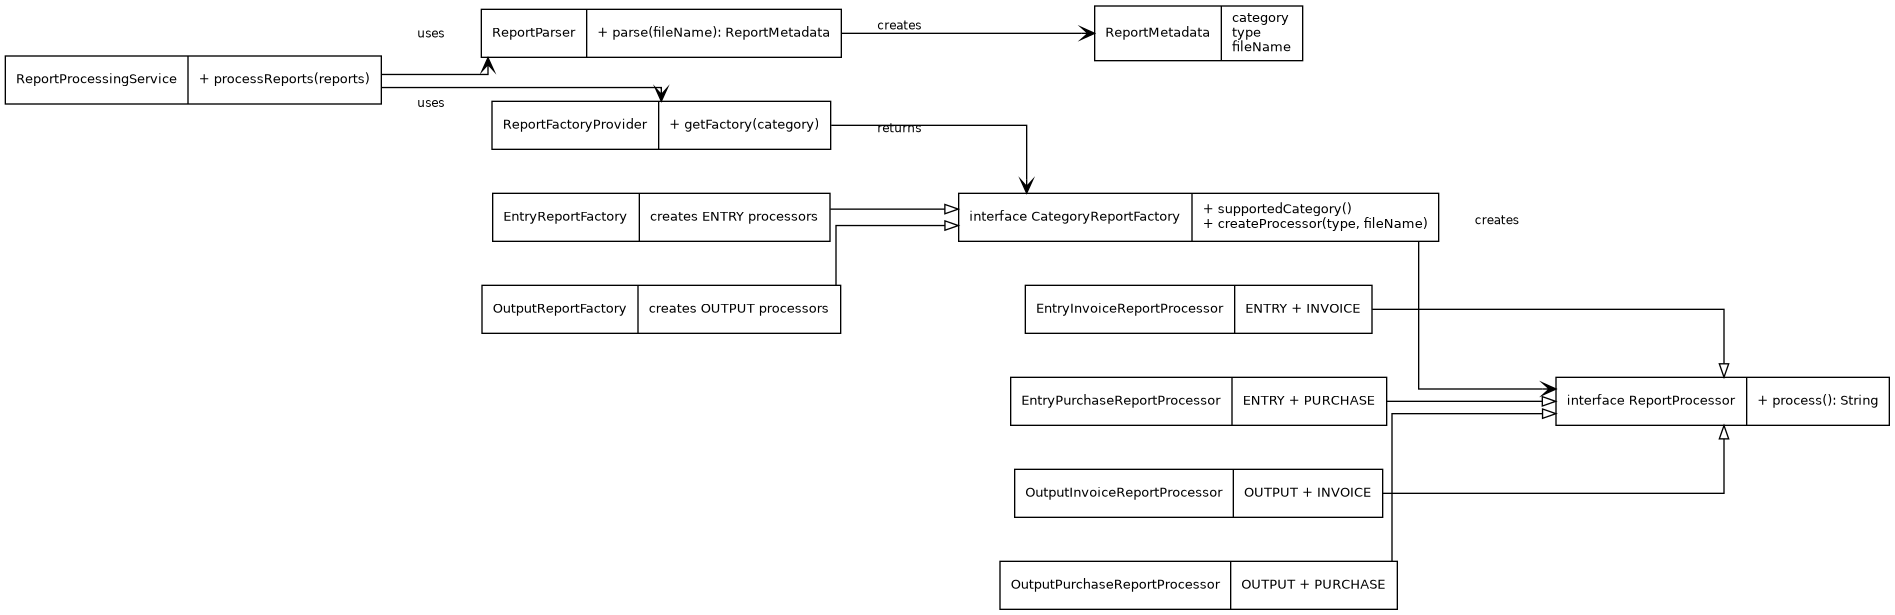
\includegraphics[width=\textwidth]{images/uml-base.png}
\caption{Diseño base del sistema con \emph{Abstract Factory}.}
\label{fig:base}
\end{figure}

\subsection{Estructura principal del código}
La interfaz abstracta de factoría mantiene una responsabilidad muy clara: crear procesadores para una familia concreta.

\lstinputlisting[style=javaStyle, caption={Interfaz de la factoría abstracta.}]{../java/src/main/java/com/unir/reuse/reports/CategoryReportFactory.java}

Sobre esa interfaz se apoya una implementación base con registro interno. Este punto es relevante porque permite que la familia \texttt{ENTRADA} soporte \texttt{PEDIDO} sin obligar a cambiar el contrato público.

\lstinputlisting[style=javaStyle, caption={Factoría abstracta con registro por tipo.}]{../java/src/main/java/com/unir/reuse/reports/AbstractMapBackedReportFactory.java}

El servicio de aplicación queda desacoplado de las clases concretas y solo orquesta el flujo principal:

\lstinputlisting[style=javaStyle, caption={Servicio de aplicación.}]{../java/src/main/java/com/unir/reuse/reports/ReportProcessingService.java}

La ejecución de prueba obligatoria se implementa mediante un \texttt{main} explícito:

\lstinputlisting[style=javaStyle, caption={Punto de entrada y prueba de funcionamiento.}]{../java/src/main/java/com/unir/reuse/reports/Main.java}

\subsection{Resultado de la simulación}
La salida por consola verifica tanto los casos válidos como una combinación no soportada:

\lstinputlisting[
  basicstyle=\ttfamily\small,
  backgroundcolor=\color{codebg},
  frame=single,
  caption={Salida generada por la ejecución del programa Java.}
]{sample-output.txt}

\section{Ejercicio 3: evolución y análisis}
\subsection{Nueva categoría MIXTA}
La primera evolución incorpora la familia \texttt{MIXTA}. El impacto estructural es limitado:

\begin{itemize}[leftmargin=*]
  \item se añade \texttt{MixedReportFactory};
  \item se incorporan dos productos concretos: \texttt{MixedInvoiceReportProcessor} y \texttt{MixedPurchaseReportProcessor};
  \item el cliente no cambia, porque sigue trabajando con la abstracción.
\end{itemize}

\begin{figure}[H]
\centering
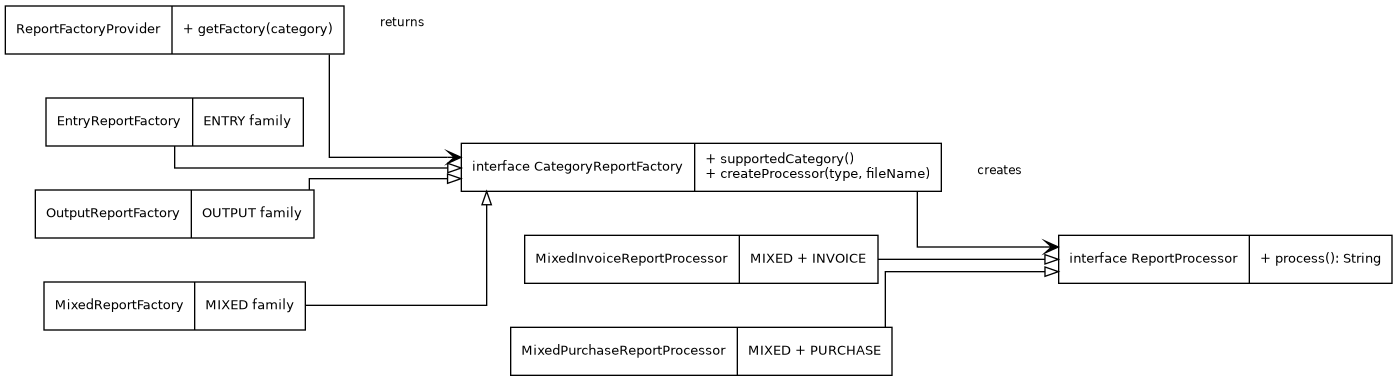
\includegraphics[width=0.95\textwidth]{images/uml-mixed-evolution.png}
\caption{Ampliación del diseño al añadir la categoría MIXTA.}
\end{figure}

\subsection{Nuevo tipo PEDIDO en ENTRADA}
La segunda evolución es más interesante desde el punto de vista del patrón, porque el nuevo tipo no aparece en todas las categorías. En una implementación estricta de \emph{Abstract Factory}, esto forzaría cambios en la interfaz abstracta y en todas las factorías concretas. En la solución adoptada:

\begin{itemize}[leftmargin=*]
  \item se añade el nuevo valor \texttt{ORDER} en la enumeración de tipos;
  \item se crea \texttt{EntryOrderReportProcessor};
  \item solo \texttt{EntryReportFactory} registra ese nuevo producto;
  \item el resto de familias permanece intacto.
\end{itemize}

\begin{figure}[H]
\centering
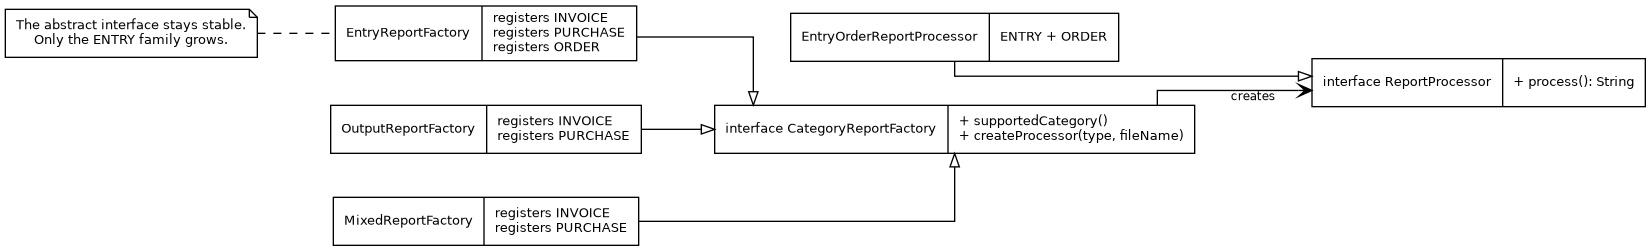
\includegraphics[width=0.92\textwidth]{images/uml-order-evolution.png}
\caption{Ampliación del diseño al añadir el tipo PEDIDO en ENTRADA.}
\end{figure}

\subsection{Valoración de la evolución}
La solución confirma dos ideas relevantes. Primero, el patrón ayuda claramente cuando se añaden nuevas familias completas, como \texttt{MIXTA}. Segundo, cuando la evolución introduce un producto asimétrico, la implementación concreta del patrón importa tanto como el patrón en sí. La variante basada en registro conserva las ventajas de \emph{Abstract Factory} y evita un coste de cambio innecesario, lo que mejora la reutilización y la mantenibilidad \cite{bloch2018effective,martin2018clean}.

\section{Conclusiones}
El uso de \emph{Abstract Factory} resulta adecuado para este problema porque el sistema procesa combinaciones de productos relacionados y, además, el enunciado exige justificar su evolución con cambios mínimos. Frente a una implementación sin patrón, la solución propuesta reduce acoplamiento, mejora la organización del código y hace más evidente dónde deben incorporarse las nuevas variantes del dominio.

La práctica también muestra una lección importante: aplicar un patrón no debe significar copiar una plantilla rígida. En este caso, una adaptación razonada de \emph{Abstract Factory} ofrece un mejor equilibrio entre pureza teórica y coste real de mantenimiento.

\bibliographystyle{plain}
\bibliography{bib/references}

\end{document}
